\documentclass{beamer}
% \usepackage[authoryear]{natbib}
\setbeamertemplate{caption}[numbered]
\usepackage{graphicx}
\graphicspath{/home/evo/4m_final_project}
\usepackage{amsmath,amsthm,amssymb}
\usepackage{verbatim}
\usepackage{times}
\usepackage[sc]{mathpazo} % Use the Palatino font
\usepackage[T1]{fontenc} % Use 8-bit encoding that has 256 glyphs
\usepackage{subcaption}
\usepackage{caption}
\captionsetup[subfigure]{labelformat=empty} % Removes the (a), (b) labels
\usepackage{hyperref}


%Information to be included in the title page:
\title{Multivariate Analysis Of The Diabetes Dataset}
\author{Rayyan Kazim, Safi Khan, Xinyi Chen, Tony Xu, Zesen Chen}
\institute{McMaster University}
\date{12/2/2024}

\begin{document}

\frame{\titlepage}

\begin{frame}
\frametitle{Dataset, Exploratory Data Analysis (EDA), Data Preparation}
\begin{itemize}
    \setlength\itemsep{1em}
    \item Using the `R` programming language, we study the diabetes dataset obtained from Kaggle which has 768 rows and 9 columns. Each row corresponds to an unique patient record, and each of the columns represent the unique variables. 
    \item There is one binary response variable that denotes presence of diabetes, the others are predictor variables. Each of the predictors are integers except for "BMI" and "DiabetesPedigreeFunction" which are categorized as float variables.
    \item The full dataset will be utilized and scaled. 75\% of the data will be used for training, and the rest will be used for testing.
\end{itemize}
\end{frame}

% \begin{frame}
%     \frametitle{Exploratory Data Analysis (EDA) and data preparation}
%     %insert all our tables
%     \begin{itemize}
%         \setlength\itemsep{1em}
%         \item All variables are integers except for "BMI" and "DiabetesPedigreeFunction"

%         \item The dataset will be split into 2, with the response variable being "outcome" and all other variables being predictor variables.
%         \item 75 percent of the data will be used for training, and the rest will be used for testing.
%     \end{itemize}
% \end{frame}

\begin{frame}
    \frametitle{EDA Continued}
	\begin{figure}[h!]
		\centering
		% First figure
		\begin{minipage}{0.48\textwidth}
			\fbox{{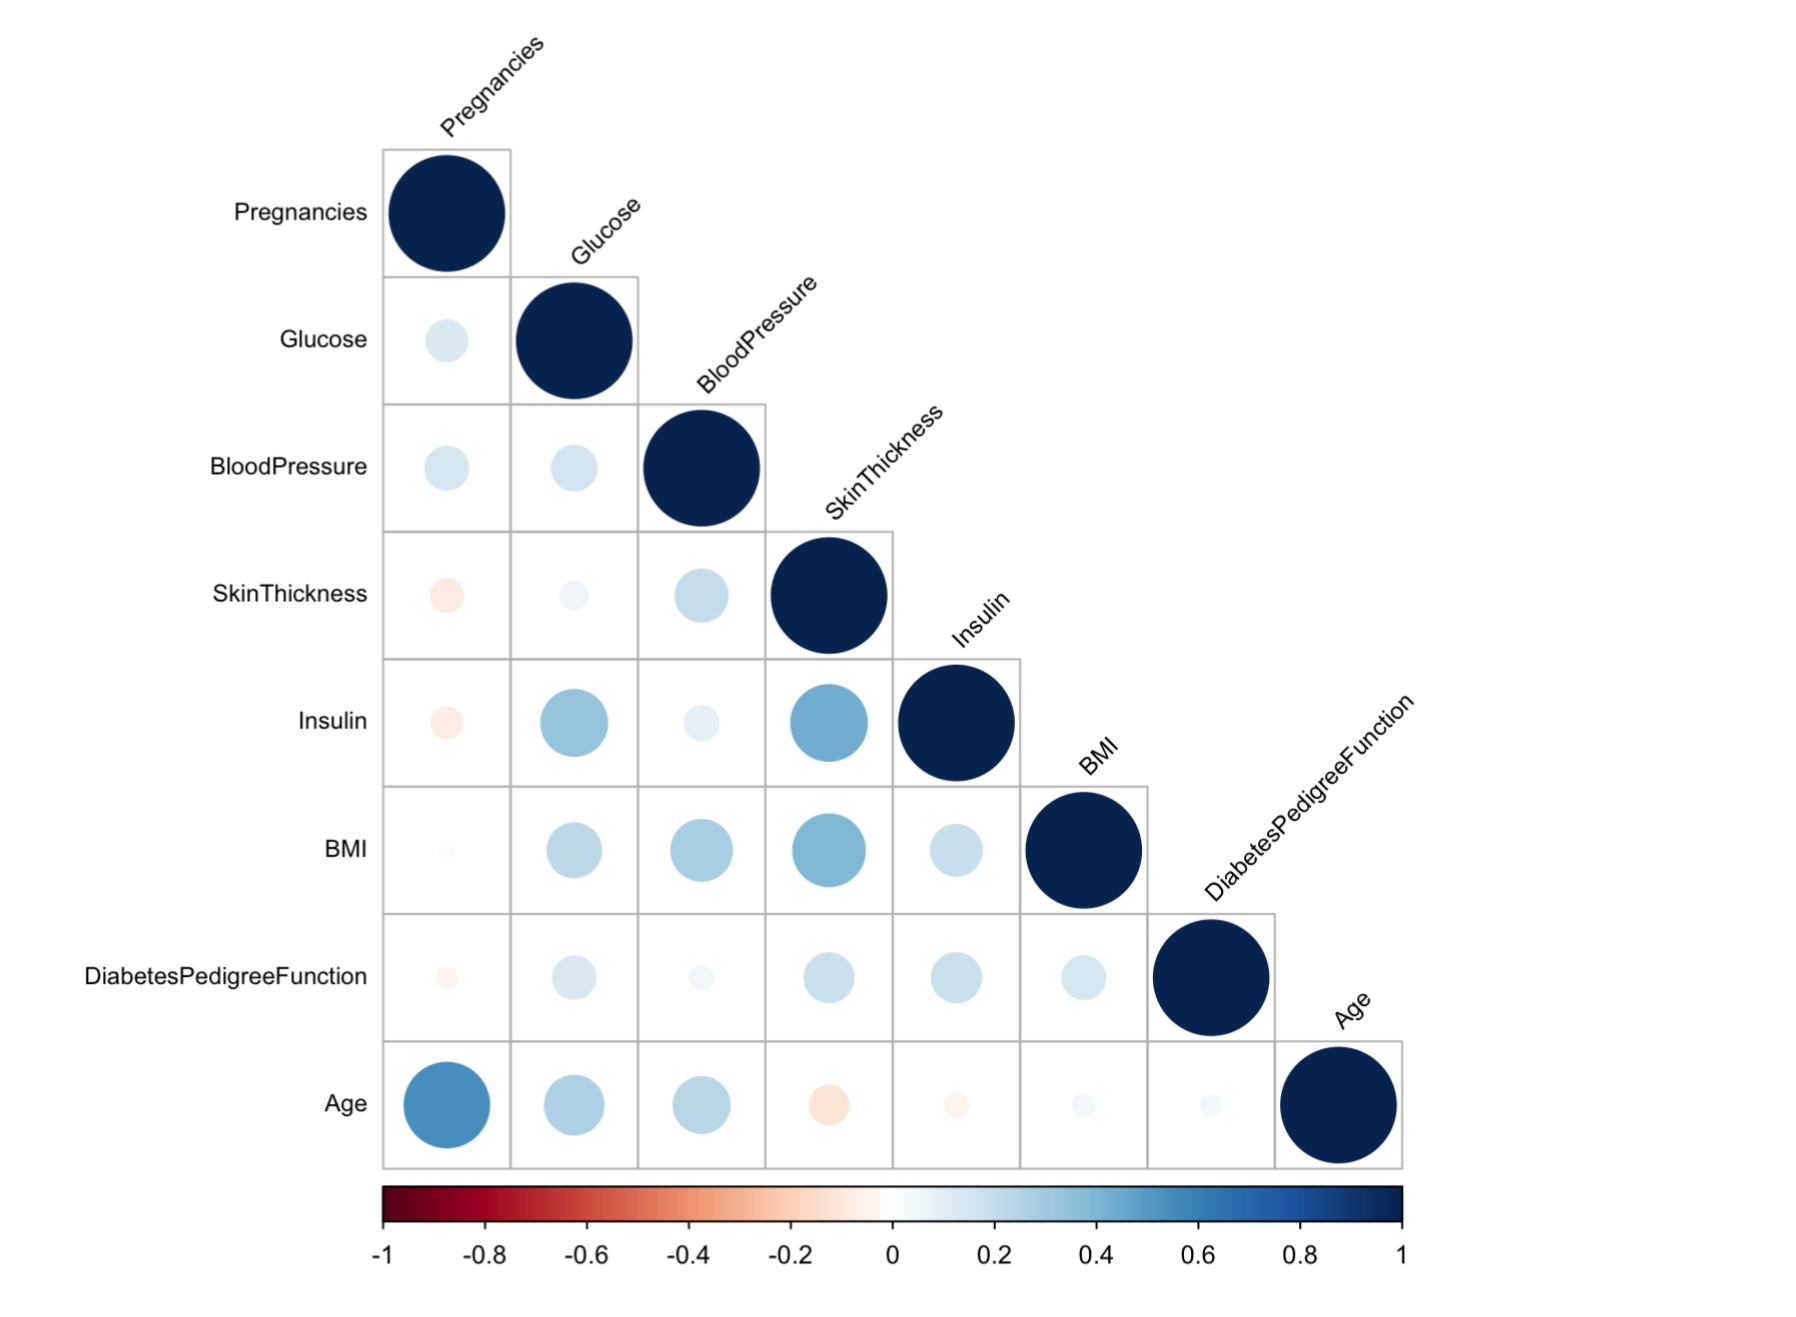
\includegraphics[width=\textwidth]{correlations2.png}}}
			\caption{Correlation of Variables} 
			\label{fig:corplot}
		\end{minipage}
		\hfill % Horizontal space between figures
		% Second figure
		\centering
		\begin{minipage}{0.48\textwidth}
			\centering
			\fbox{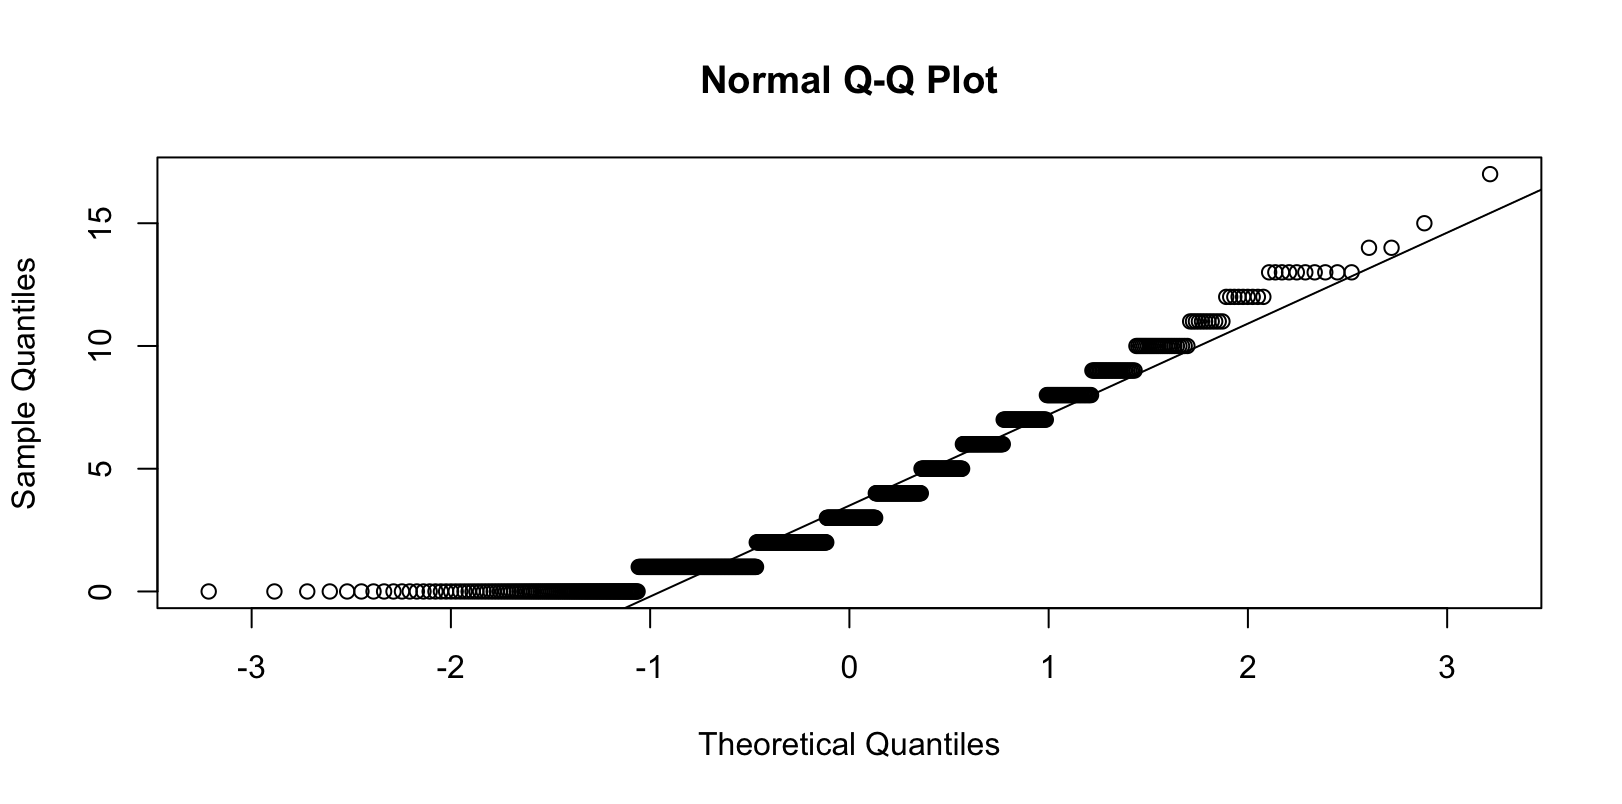
\includegraphics[width=\textwidth]{normal.png}} 
			\caption{Normal QQ-Plot} 
			\label{fig:qqplot}
		\end{minipage}
	\end{figure}
	\vspace{-0.2cm} % Reduce space between text and figure
    \begin{itemize}
        \item Figure~\ref{fig:corplot} showcases that "SkinThickness" is well correlated with "BMI" and "Insulin," while "Age" is well correlated with "Pregnancies." Additionally, "Glucose" is reasonably correlated with "insulin," "BMI," and "Age."
        \item Figure~\ref{fig:qqplot} indicates that our dataset is not normally distributed.
    \end{itemize}
    
\end{frame}

\begin{frame}
    \frametitle{Methodologies - Supervised Learning Analysis}
        \begin{itemize}
            \setlength\itemsep{1em}
            \item Used the following Supervised Learning Analysis methods: k-Nearest Neighbours (k-NN), Random Forest, and Boosting to study our dataset.
            \item k-NN is a non-parametric, supervised learning classifier that uses proximity to make classifications about the grouping of a dataset.
            \item Random Forest is a bootstrapping sampling method that combines the results of multiple decision trees to draw on a conclusion.
            \item Boosting is similar to Random Forest, however it is not a bootstrapping sampling method. Boosting also uses the entire dataset, or some subsample thereof, to generate the ensemble.
        \end{itemize}
\end{frame}

\begin{frame}
    \frametitle{Methodologies - Binary Logistic Regression}
        \begin{itemize}
            \setlength\itemsep{1em}
            \item We performed Binary Logistic Regression because the response variable of our dataset, "Outcome," is binary.
            \item The initial model incorporates all eight predictor variables.
            \item The objective of using this technique is to identify the most significant predictors by using backwards elimination.
            \item This process ensures the final model will have only the most significant variables.
        \end{itemize}
\end{frame}

% \begin{frame}
%     \frametitle{Discussions - Logistic regression}
%         \begin{itemize}
%             \setlength\itemsep{1em}
%             \item Table ~\ref{tab:BinLogReg} suggests that we should remove variables "SkinThickness" and "insulin" from the model, since their p-values were greater than $0.05$.
%             \item Table ~\ref{tab:BinLogRegA} implies that we have sufficient evidence to suggest that "Pregnancies", "Glucose", "Blood Pressure", "BMI", "DiabetesPedigreeFunction" and "Age" have a significant influence over "outcome". 
%             \item We obtain that the MCR for binary logistic regression is $0.23958$.
%         \end{itemize}
% \end{frame}

\begin{frame}
    \frametitle{Discussion - Binary Logistic Regression}
        \begin{itemize}
            \setlength\itemsep{1em}
            \item Table~\ref{tab:BinLogReg} illustrates that "BloodPressure," "SkinThickness," "Insulin," and "Age," are statistically insignificant because their $p-$values are greater than $\alpha = 0.05$ level of significance, indicating that they should be removed in the final model. 
            \end{itemize}
 \begin{table}[h!]
        \centering
        \resizebox{=0.92\textwidth}{!}{
            \begin{tabular}{|l|l|l|l|l|}
                \hline
                \textbf{Coefficients} & \textbf{Estimate} & \textbf{Std. Error} & \textbf{Z-Value} & \textbf{Pr(>|Z|)} \\ \hline
                (Intercept) & -0.863576 & 0.111504 & -7.745 & 9.57E-15 \\ \hline
                Pregnancies & 0.411598 & 0.128257 & 3.209 & 1.33E-03 \\ \hline
                Glucose & 1.003291 & 0.133428 & 7.519 & 5.51E-14 \\ \hline
                BloodPressure & -0.15522 & 0.122145 & -1.271 & 0.2038 \\ \hline
                SkinThickness & -0.008376 & 0.123519 & -0.068 & 0.94594 \\ \hline
                Insulin & -0.160385 & 0.120504 & -1.331 & 1.83E-01 \\ \hline
                BMI & 0.699525 & 0.135793 & 5.151 & 2.59E-07 \\ \hline
                DiabetesPedigreeFunction & 0.295516 & 0.114215 & 2.587 & 0.00967 \\ \hline
                Age & 0.212147 & 0.127142 & 1.669 & 0.0952 \\ \hline
            \end{tabular}
        }
        \caption{Binary Logistic Regression Full Model Output}
        \label{tab:BinLogReg}
    \end{table}    
\end{frame}
\begin{frame}
    \frametitle{Discussion - Binary Logistic Regression Continued}
    \begin{itemize}
        \item The $p-$values from Table~\ref{tab:BinLogRegA} imply we have sufficient statistical evidence to conclude the variables present in the model have a significant influence in predicting "Outcome."
    \end{itemize}
    \begin{itemize}
        \item Table~\ref{tab:BinLogRegA} highlights Odds Ratio values of each predictor, showcasing the highers odds each variable has on predicting a  positive or non-positive outcome. 
    \end{itemize}
    \vspace{-0.3cm} % Reduce space between text and figure
    \begin{table}
        \centering
        \resizebox{=\textwidth}{!}{
            \begin{tabular}{|l|l|l|l|l||l|}
                \hline
                Coefficients: & Estimate & Std. Error & z value & Pr(>|z|) & Odds Ratio \\ \hline
                (Intercept)   & -8.118918 & 0.730397 & -11.116 & <2e-16 & --- \\ \hline
                Pregnancies   & 0.154186  & 0.032151 & 4.796   & 1.62E-06 & 1.167 \\ \hline
                Glucose       & 0.030679  & 0.003781 & 8.113   & 4.92e-16 & 1.031 \\ \hline
                BMI           & 0.080086  & 0.016048 & 4.990   & 6.03e-07 & 1.083 \\ \hline
                DiabetesPedigreeFunction & 0.863621 & 0.336274 & 2.568 & 0.0102 & 2.372 \\
                \hline
            \end{tabular}
        }
        \caption{Binary Logistic Regression Reduced Model Output with Odds Ratio}
        \label{tab:BinLogRegA}
    \end{table}
    \vspace{-0.5cm} % Reduce space between text and figure
    \begin{itemize}
        \item We obtain that the MCR for binary logistic regression is $0.23958.$
    \end{itemize}
\end{frame}



\begin{frame}
    \frametitle{Discussion - k-Nearest Neighbours}
    %insert the plot here.
        \begin{itemize}
            \setlength\itemsep{1em}
            \item Figure~\ref{fig:KNNPlot} highlights that tuning with 5-fold cross validation suggests that the best value for $k$ is $3$.
            \item Running the k-NN algorithm with $k=3$, we conclude that the MCR $=$ $0.2916667.$
        \end{itemize}
        \begin{figure}[h!]
            \centering
            \fbox{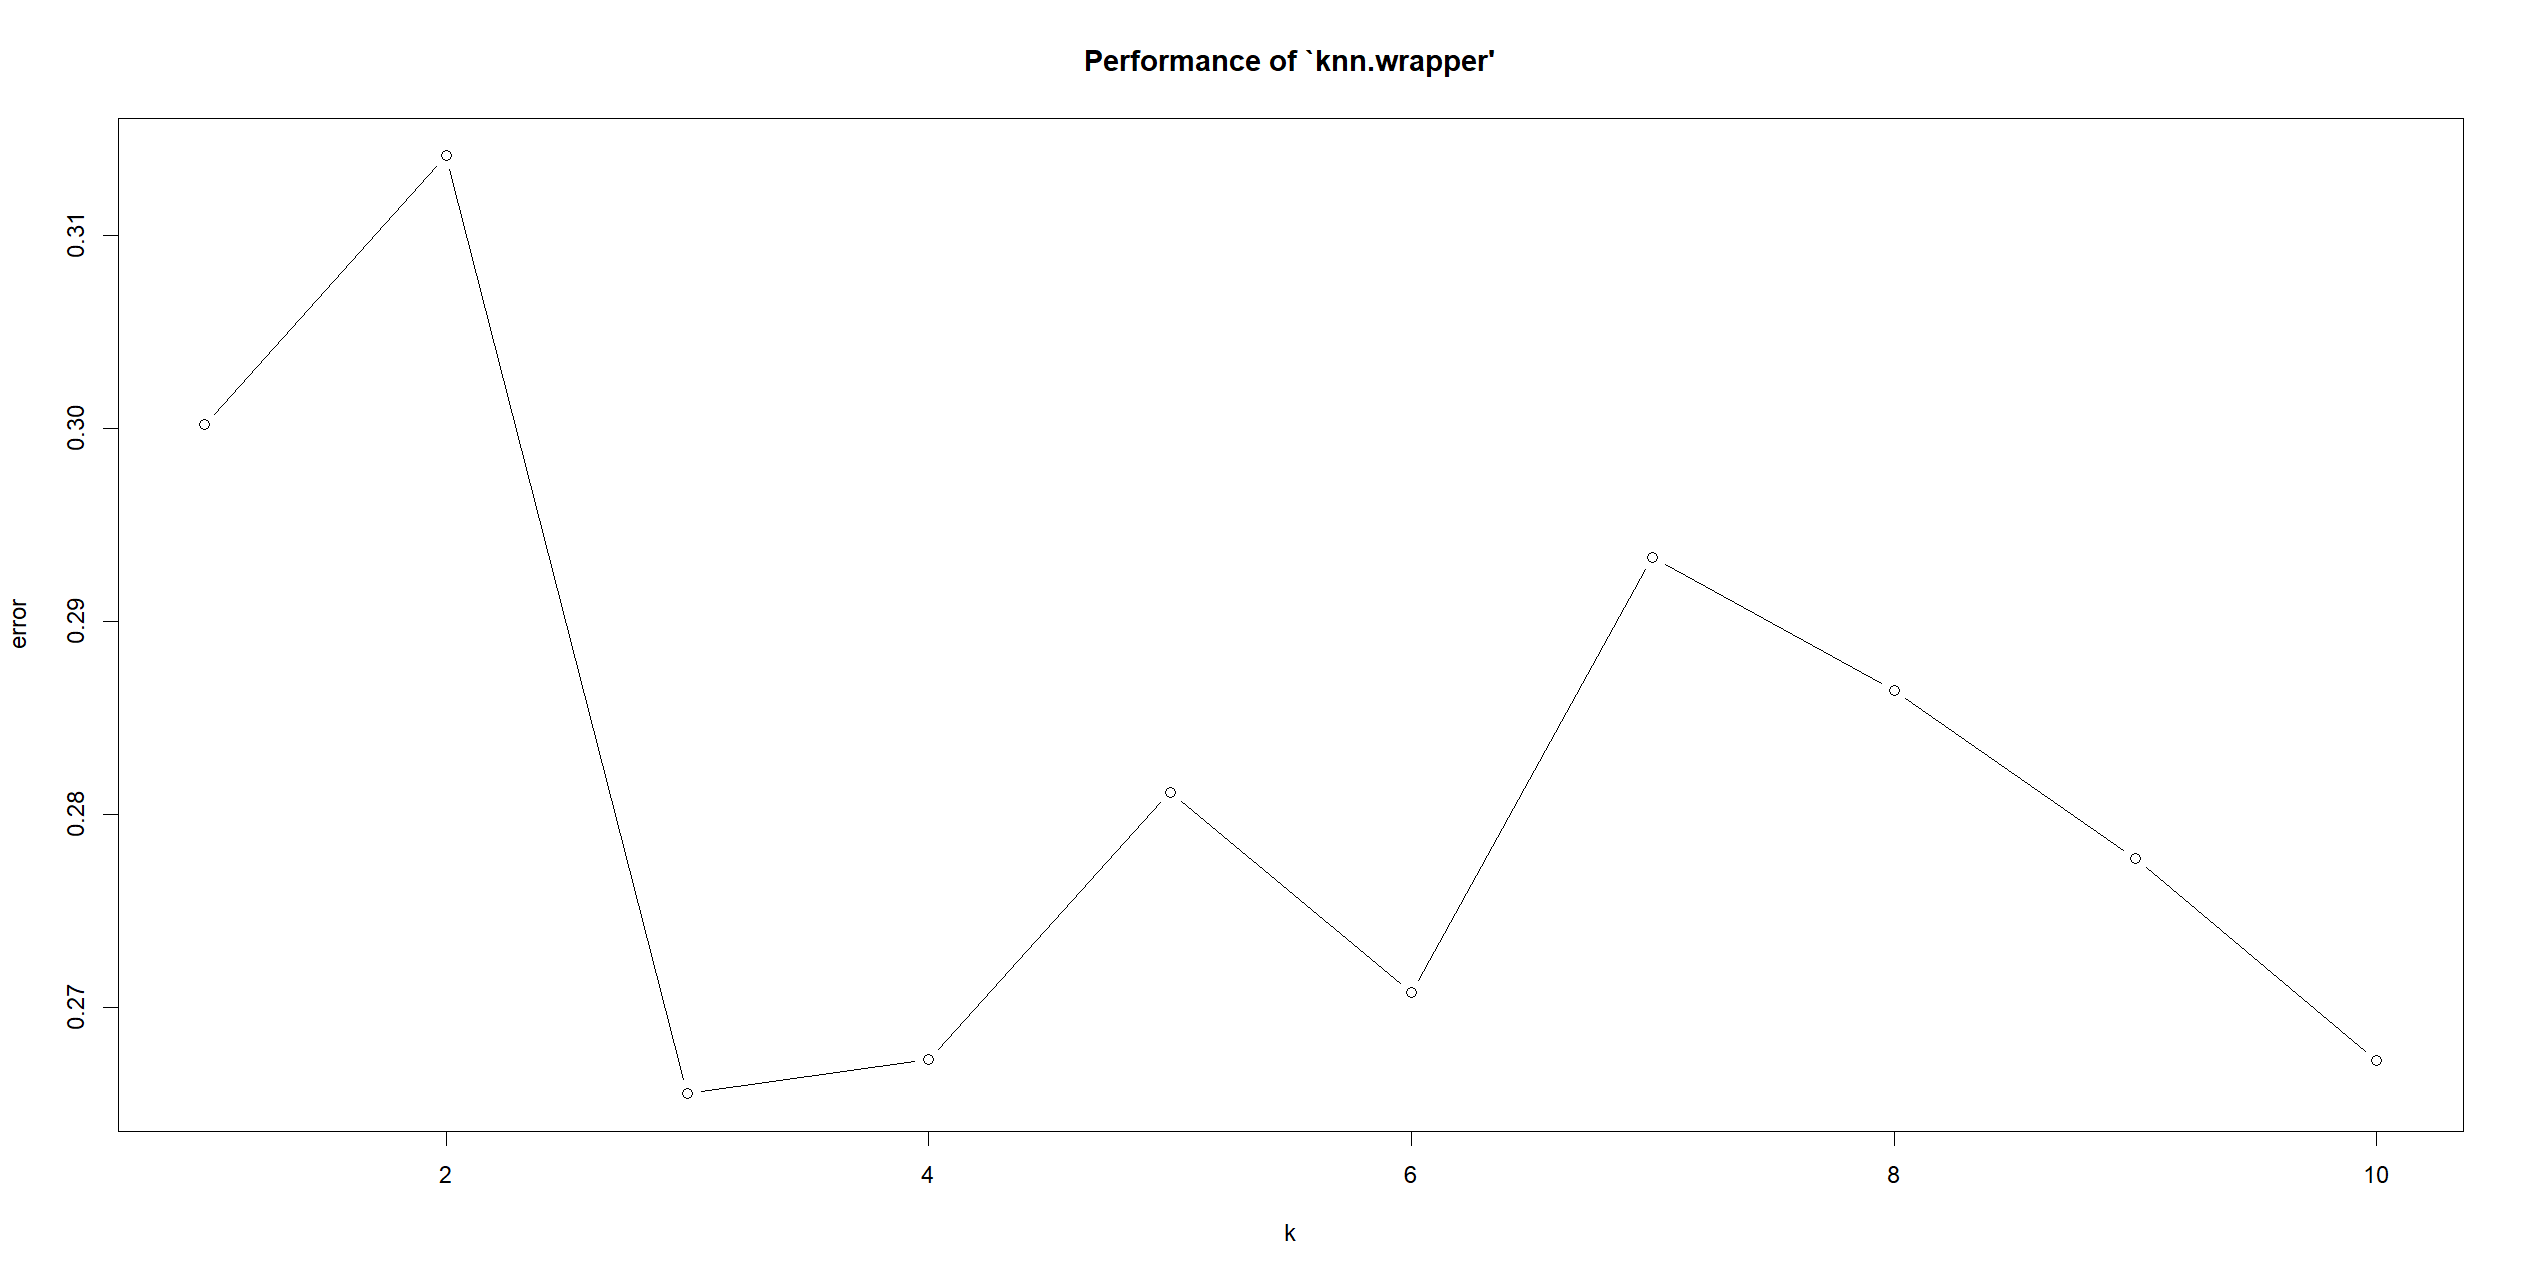
\includegraphics[width=0.80\textwidth]{knnplot.png}} 
            \caption{Output Plot From k-NN Classification} 
            \label{fig:KNNPlot}
        \end{figure}
\end{frame}

\begin{frame}
    \frametitle{Discussion - Random Forest}
    %insert the variable importance plot here.
        \begin{itemize}
            \setlength\itemsep{1em}
            \item Tuning with 5-fold cross validation gives the best value for $\mathcal{M}$ and $M$ as $4$ and $200$ respectively.
            \vspace{-0.2cm} % Reduce space between text and figure
            \item Running Random Forest with $\mathcal{M} = 4$ and $M = 200$, we conclude that the MCR $ = 0.28125.$
            \vspace{-0.2cm} % Reduce space between text and figure
            \item Figure~\ref{fig:RFPlot} showcases that "Glucose" and "BMI" are the two most important variables in the model.
        \end{itemize}
        \begin{figure}[h!]
            \centering
            % First figure
            \fbox{{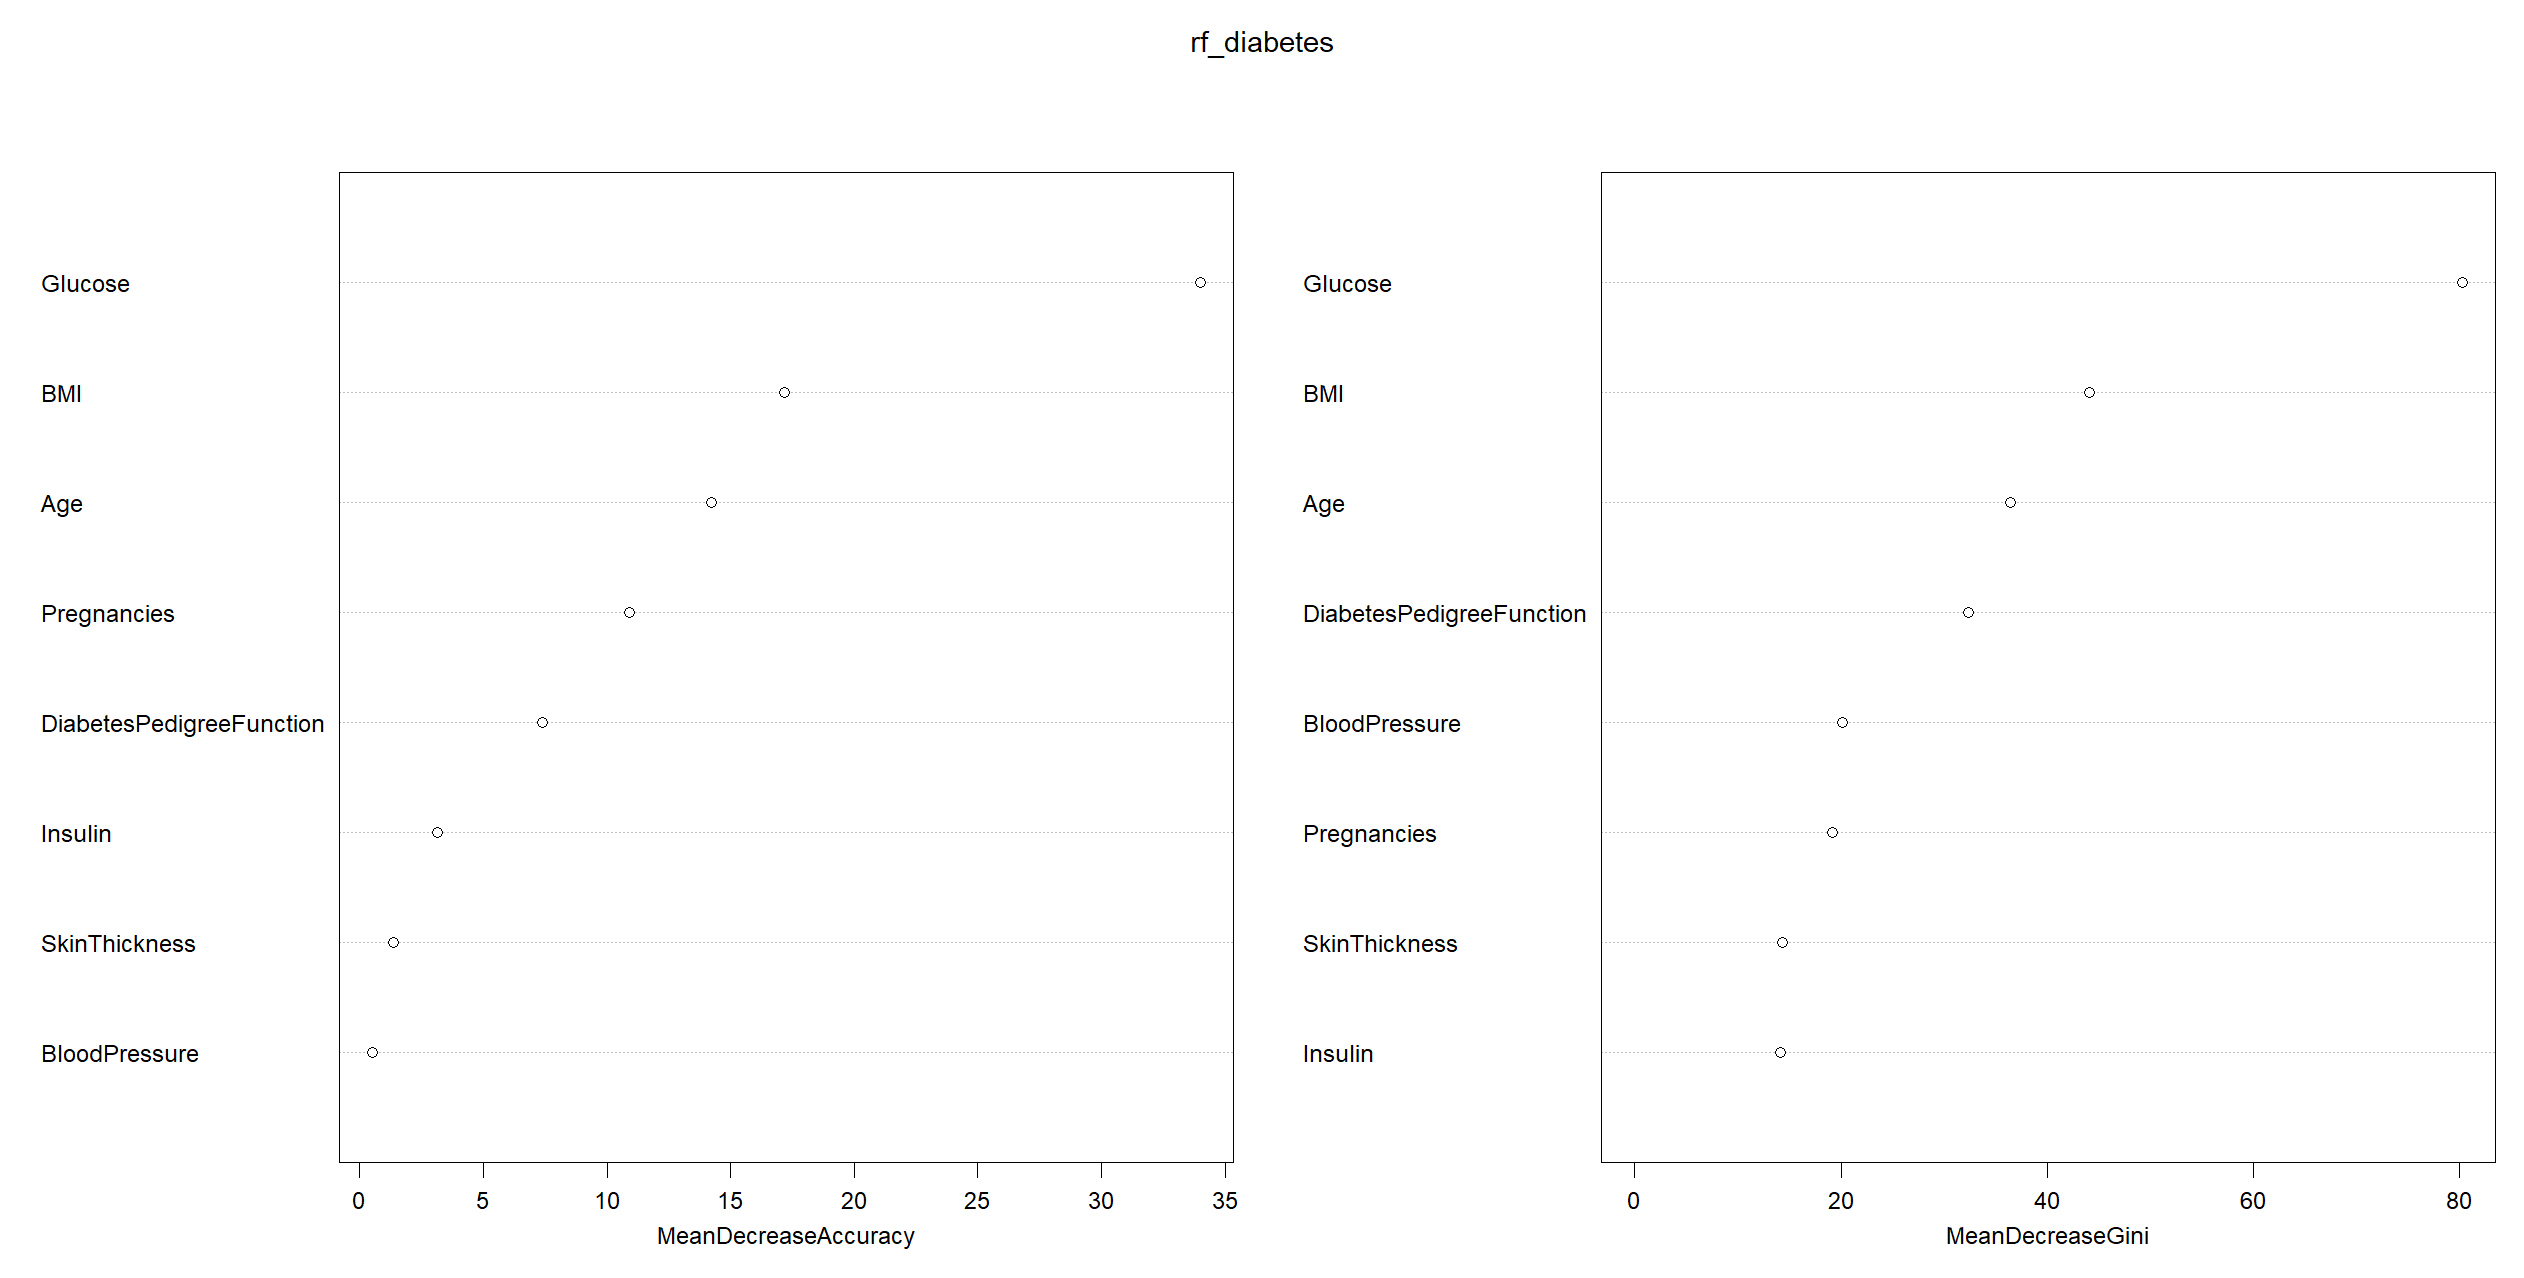
\includegraphics[width=0.78\textwidth]{MeanDecreaseAccuracyPlotForRandomForest.png}}}
            \caption{Random Forest Variable Importance} 
            \label{fig:RFPlot}
        \end{figure}
\end{frame}

\begin{frame}
    \frametitle{Discussion - Boosting}
    \begin{itemize}
        \item Boosting achieved an accuracy of $73.44\%$ (an MCR of $0.2656$), and an AUC of $0.802$. 
        \item Figure~\ref{fig:importance} identifies "Glucose," "BMI," and "Age" as the most most predictors for "Outcome" in our Boosting model.
    \end{itemize}
    \begin{figure}[h!]
        \centering
        % First figure
        \begin{minipage}{0.48\textwidth}
            \fbox{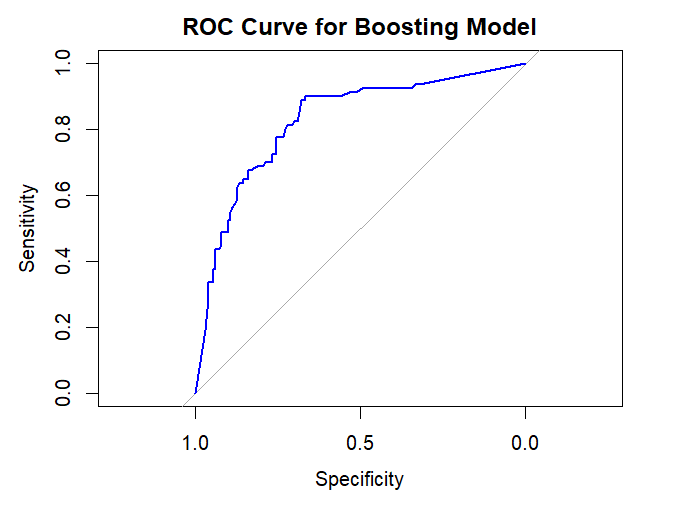
\includegraphics[width=\textwidth]{G2.png}} 
            \caption{ROC Curve for Boosting Model} 
            \label{fig:ROC curve}
        \end{minipage}
        \hfill % Horizontal space between figures
        % Second figure
        \centering
        \begin{minipage}{0.48\textwidth}
            \centering
            \fbox{{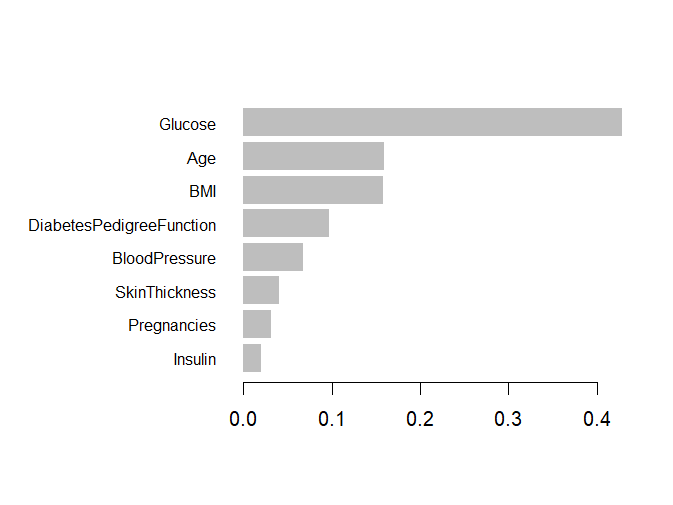
\includegraphics[width=\textwidth]{G1.png}}}
            \caption{Age Feature importance plot} 
            \label{fig:importance}
        \end{minipage}
    \end{figure}
\end{frame}
   
\begin{frame}
    \frametitle{Conclusion}
    %insert the variable importance plot here.
        \begin{itemize}
            \item The MCR values of each method indicate that Binary Logistic Regression was the most accurate out of all methods used.
            \item We effectively showcased
            the performance accuracy of the k-Nearest Neighbours algorithm, Binary Logistic Regression algorithm, and the ensemble methods: Random Forest and Boosting. 
            \item The conclusions
            determined by each of the various methods align with the general scientific consensus on predictors for diabetes.
        \end{itemize}
\end{frame}

    % \begin{frame}
    %     \frametitle{References}
    %     \bibliographystyle{apa} 
    %     \bibliography{references}
    % \end{frame}

\end{document}
